%% inicio, la clase del documento es iccmemoria.cls
\documentclass{iccmemoria}
\usepackage{amsmath}
\usepackage{algorithm}
\usepackage{tabularx}
\usepackage[noend]{algpseudocode}

\algdef{SE}[DOWHILE]{Do}{doWhile}{\algorithmicdo}[1]{\algorithmicwhile\ #1}%


%% datos generales y para la tapa
\titulo{Análisis experimental de IIQS para extender el soporte a secuencias de elementos repetidos}
\tituloEng{Experimental analysis of (I)IQS to fine-tune support for arrays with repeated elements}
\author{Erik Andrés Regla Torres}
\supervisor{Rodrigo Andrés Paredes Moraleda}
\informantes
	{NN 1}
	{NN 2}
%\adicional{(sólo por si se necesita agregar algún otro profesor)}
%\director{Profesor del ramo Memoria de Título} % no entiendo para que esta esto :-(
%innocuous comment :-p
%cambio 2
\date{mes, año}

%% inicio de documento
\begin{document}

%% crea la tapa
\maketitle
%cambio 5
%cambio 3
%cambio 4

%% dedicatoria
\begin{dedicatory}
  Dedicated to... someone ?
\end{dedicatory}

%% agradecimientos
\begin{acknowledgment}
  Agradecimientos a ... (how the fuck do I choose whom to acknowledge?)
\end{acknowledgment}

%% indices
\tableofcontents
\listoffigures
\listoftables

%% resumen
\begin{resumen}
  I'm gonna write the summary as the last part.
\end{resumen}

%% abstract

%% contenido del primer capítulo
%% This should be the last thing to write
\chapter{Introduction}
Aquí va el texto del capítulo 1...

\section{Context}
Aquí va el texto de la primera sección del capítulo 1...

\section{Application areas}
Aquí va el texto de la primera subsección de la primera sección del capítulo 1...

\section{Problem description}
Aquí va el texto de la segunda subsección de la primera sección del capítulo 1...

\section{Goals}
Aquí va el texto de la segunda subsección de la primera sección del capítulo 1...

\subsection{General goals}
Aquí va el texto de la segunda subsección de la primera sección del capítulo 1...

\subsection{Specific goals}
Aquí va el texto de la segunda subsección de la primera sección del capítulo 1...

\section{Document Structure}
Aquí va el texto de la segunda subsección de la primera sección del capítulo 1...

\chapter{Pilot experiments}

\section{Experimental Setup}


\section{Base benchmarking}
In experimental algorithms, the first step before engaging into a optimization job is to benchmark our current solutions in order to formulate our hypothesis and expectations. In this case we will check the behaivour of base implementations IQS and IIQS to understand better what IQS and IIQS is, what is happening when a worst case arises and to devise the next steps of this experimental development.

\subsection{Average and worst case}
RESULTS, A TON OF CHARTS AND DISCUSSION
\subsection{Influence of presortedness}
RESULTS, A TON OF CHARTS AND DISCUSSION
\subsection{Influence of repeated elements}
RESULTS, A TON OF CHARTS AND DISCUSSION



% REMEMBER TO ANSWER THEESE QUESTIONS:

% Is IIQS execution for repeated elements an instance of IQS worstcase?
% Does presortedness affect (I)IQS running time?
% Does the size of the elements stored in the stack affect its performance?
% It is worth to use iterative versions of BFPRT as approximate median selection?
% Are the average cases for repeated and non repeated classes the same?} %rewrit
% Can we tune (I)IQS to support repeated cases without affecting its average running time?
\section{Partitioning Schemes}

\subsection{Rationale}
Before diving into the results for this experiment, we will now explain two partition strategies to take into consideration before designing our first experiment and our second algorithm modification in order to understand the modifications made to IQS.

\subsection{Partition schemes}
As explained before in~\ref{SEC:INCREMENTAL_SORTING}, partition algorithms play a fundamental role on sorting algorithms like QuickSort. But partition algorithms can use different schemes in order to partition the array into two sections, depending on which properties of the process we want to optimise.

\subsection{Lomuto's partition scheme}

The most identificable feature of this algorithm is that it uses the last element as the pivot for partitioning the array, which makes suitable for shuffled sequences but when the sequence follows some of the first disorder metrics seen in~\ref{SEC:MEASURING_DISORDER} it tends to bias the performance of this partition scheme.

This algorithm is commonly referenced as the easiest way to partition an array, given it is low complexity.
o
\begin{algorithm}
\caption{Lomuto Partition}\label{ALG:LOMUTO_PARTITION}
\begin{algorithmic}[1]
    \Procedure{$lomuto$}{$A, p, r$}
    \State $x \gets A_r$
    \State $i \gets p-1$
    \For{$j \in [p, r - 1]$}
    \If{$A_j \leq x$}
        \State $i \gets i + i$
        \State $swap(A_i, A_j)$
    \EndIf
    \EndFor
    \State $swap(A_{i+1}, A_r)$
    \State \Return $i + 1$
    \EndProcedure
\end{algorithmic}
\end{algorithm}

\subsection{Hoare's partition scheme}
Hoare's partition scheme takes another approach at partitioning elements by using two indices which converge into the postition of the pivot chosen at the beggining. When it comes to sort a set of elements it works faster than Lomuto's implementation and it's more stable. and given that the pivot can be chosen randomly, the introduction of randomness helps to ease biased pivot selections.

\begin{algorithm}
\caption{Hoare's Partition}\label{ALG:HOARE_PARTITION}
\begin{algorithmic}[1]
    \Procedure{$hoare$}{$A, p, r$}
    \State $x \gets A_p$
    \State $i \gets p-1$
    \State $j \gets r+1$
    \While{$true$}
        \Do 
            \State $j \gets j - 1$
        \doWhile{$A_j \leq x$}

        \Do 
            \State $i \gets i + 1$
        \doWhile{$A_j \geq x$}

        \If{$i < j$}
            \State $swap(A_i, A_j)$
        \Else
            \State \Return $j$
        \EndIf
    \EndWhile
    \EndProcedure
\end{algorithmic}
\end{algorithm}

\subsection{Dutch flag problem}
Both of the aforementioned algorithms performs over sets, but when it comes to sequences, to use such partition methods fails dramatically as it treats repeated elements as unique elements. In worst case, the pivot is positioned into its corresponding place but it does not guarantee that there are no repetitions of the same element on any portion of the original sequence.

\subsection{Problem definition and solution}
Let's take as example the partitioning problem of the following two sequences:

$$ S_1={1,2,3,4,5,6,7,8,9} $$
and
$$S_2={1,2,5,5,5,5,5,8,9}$$

It's clear that if we chose $p$ equal to $5$, the element in the fifth position of $S_1$ will be the pivot on its correct place. But it's not the case for $S_2$ as we can get a pivot from the third up to the seventh position on the sequence. In this case, as all the positions are valid pivots, there is no safety guarantee that the resulting pivot will partition the array in half in order to ensure a $log_2$ decay on the problem space. Situation worsens if all the elements are repeated, as it defeats the purpose of partitioning the sequence~\cite{7416566}.

This problem is also known as the Dutch Flag problem~\cite{10.5555/550359}, which for given a sequence it partition inplace the elements lower than the pivot value, the elements equal to the pivot value and the elements greater than the pivot value and it will return the indices of the beggining and the end of the middle portion.

\begin{algorithm}
\caption{Hoare's Partition}\label{ALG:HOARE_PARTITION}
\begin{algorithmic}[1]
    \Procedure{$hoare$}{$A, p, r$}
    \State $x \gets A_p$
    \State $i \gets p-1$
    \State $j \gets r+1$
    \While{$true$}
        \Do 
            \State $j \gets j - 1$
        \doWhile{$A_j \leq x$}

        \Do 
            \State $i \gets i + 1$
        \doWhile{$A_j \geq x$}

        \If{$i < j$}
            \State $swap(A_i, A_j)$
        \Else
            \State \Return $j$
        \EndIf
    \EndWhile
    \EndProcedure
\end{algorithmic}
\end{algorithm}

\subsection{Integration into IQS as base implementation}

SECTION WITH RESULTS HERE!!!

As it can be seen, there no noticeable difference between experimental complexities of implementations for three-way partitioning and standard partitioning algorithms. As such, from now on we will use \textit{three-waw-partition} as our default implementation for the partitioning stage. This will allow us to contrast results between IQS and IIQS with such modifications using both repeated and non repeated elements as dataset inputs.







\section{Influence of pivot selection}

In this experiment we establish a baseline for selecting pivots on partition-based sorting algorithms. While it is commonly known that randomized approaches are the most effective way of dealing with unknown distributions~\cite{estivil92}, in this approach we want to confirm if by biasing the selection on the partitioning stages of the algorithms have any direct influence over its running time.

\subsection{Understanding pivot bias}

As explained before in Section~\ref{SECTION:PARTITIONING_SCHEMES}, all partition based algorithms are based in the idea of generating two equal sized partitions, which contributes to a continuous decrease by a factor of 2 on each iteration. Under normal circumstances, it is expected that $log_2(n)$ partition operations are executed for a given sequence of $n$ size.

But this assumption only yields when there is only one pivot to select. Meaning that there is a single element which divides both partitions generated by the algorithm, so for the case of a \emph{three-way-partition} it does not apply. Let us take a example of a sequence $S$ of size $n$ which contains $n$ unique integer elements. So, by induction on the integer number definition, each element if used as pivot for a partition can only yield one and only one pair of partition sets on $S$.

When repeated elements are found on $S$ we face a problem with the definition itself of partition presented in Section~\ref{SUBSECITON:PARTITIONING_PROBLEM}, as there is no guarantee that the partitioned element is present or not in the resulting array. Using a three-way partitioning element does not solve the problem of reducing the search space and in this regard we have the following two options:

\begin{itemize}
    \item Group the repeated elements and threat that set of repeated element as they were a unique element on $S$ --- we discuss this approach on Section~\ref{SECTION:STACK_STRUCTURE}.
    \item Preserve the elements into the array and we apply a set of rules to choose which element deliver as our pivot.
\end{itemize}

This makes a lot of sense when revisiting the plot at Figure~\ref{FIG:BENCHMARK_05_CLASSES}, as the more predominant is a certain class in a sequence, the less important becomes the pivot value selected but their final position.

\subsection{Effects on the partitioning}

Let us consider the pivot bias as a rational number $p_b \in [0,1]$. This bias allows us to map to indexes in $S$ to a floating point representation by assuming $S_i = \lfloor n\cdot p_{b}  \rfloor, \forall ~i~ \in[0,\norm{S}($. In colloqual terms, this means that a index of $0.0$ means that the returned pivot belongs to the leftmost index of the middle segment, a value of $0.5$ a pivot in the middle of the segment and $1.0$ the rightmost element, asumming that the elements are sorted in a ascending fashion.

\begin{figure}[!ht]
    \centering
    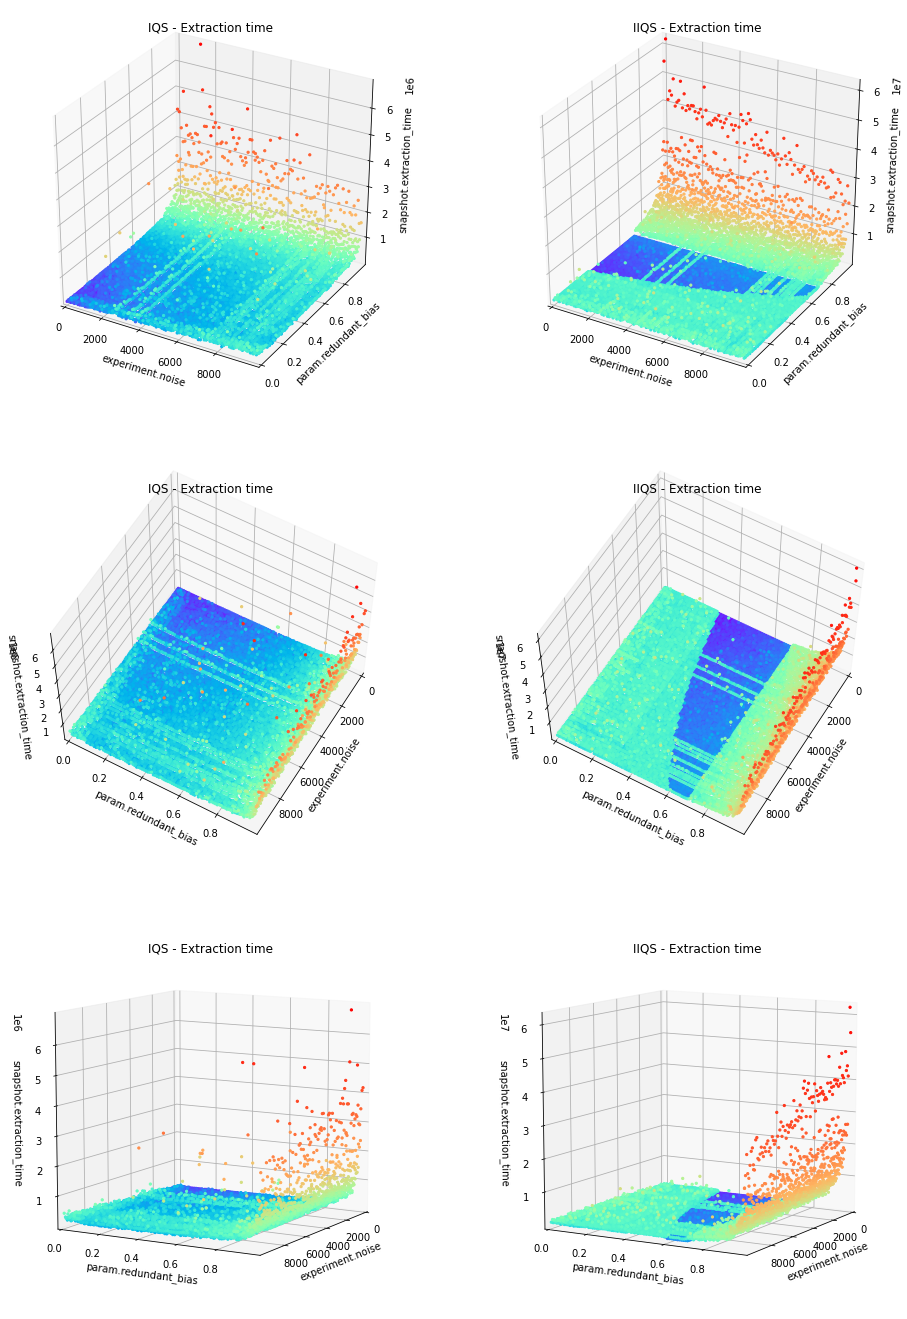
\includegraphics[width=0.8\textwidth]{./fragments/04_experimental_execution/images/01_basebenchmark_06_noise_bias.png}
    %\caption{Benchmark for random case. IQS and IIQS executions are shown on the first and second columns respectively.}
    \caption{Benchmark for randomly sorted sequence with repeated elements $1\times10^4$ elements. IQS and IIQS executions are shown on the first and second column respectively. All extractions are being shown using a linear scale.}
    \label{FIG:BENCHMARK_06_NOISE_BIAS}
\end{figure}

For our first observation we limit the result to only examine the first extraction performed by IQS, as it is already known that it is the most compute intensive operation in this algorithm. Then, we can observe in Figure \ref{FIG:BENCHMARK_06_NOISE_BIAS} that both the noise amount and the bias over the partition have a huge impact when extracting the first element in the sequence which is also different for both implementations of the algorithm.

% By examining the extra information provided by our first experiment, there are two noticeable details on the effect of biasing the selection of the resulting pivot. 
There are some interesting effects of the sequence noise for the repeating case instance. IQS shows the best performance as the noise decreases but also as the pivot bias is more inclined towards selecting the smaller elements. But this effect it is only an illusion generated by the same case depicted on Figure~\ref{FIG:BENCHMARK_02_ASC_CASE}, as less noise is found in the sequence, the greater the chance to select as pivot an element belonging to the repeating portion of the sequence, hence the bias effect studied on IQS for the partition comes into full effect. Both changing the bias towards greater values and to increase the noise contributes to increase the extraction time, it is clear that the bias has a greater effect than noise. 

Then something interesting happens on IIQS, as the behaviour is not as smooth as on IQS case. There is a valley that it appears to be in function of the bias, which for certain amounts of noise in the sequence it favours their execution. This is because of a forced execution of the introspective steps. Both noise and pivot bias have a huge impact on the times that this step is executed, hence, aditional $O(n)$ time is consumed on the iteration when the noise exceeds IIQS fixed $\alpha$ and $\beta$ constraints~\cite{7416566}. In the same fashion as our previous observations, the fact that this effect decreases when inducing more noise is related to the probability of randomly selecting a pivot which belong to a repeated portion of the array. When this happens we notice a great reduction of the running time, which suggest that we should adjust our pivot bias to match our $\alpha$ and $\beta$ values in order to get the best performance.

\begin{figure}[!ht]
    \centering
    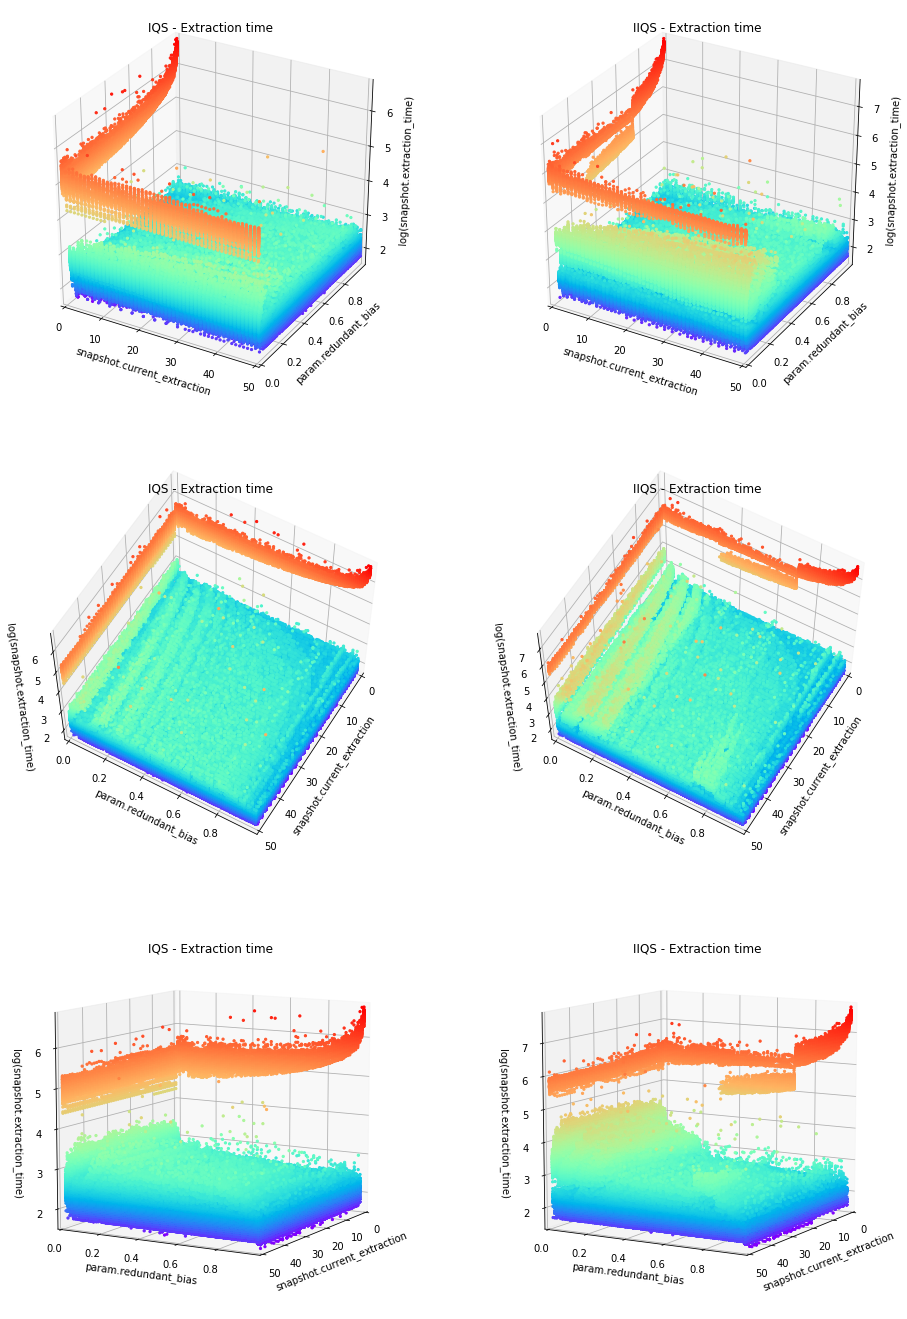
\includegraphics[width=0.8\textwidth]{./fragments/04_experimental_execution/images/01_basebenchmark_07_extraction_bias.png}
    %\caption{Benchmark for random case. IQS and IIQS executions are shown on the first and second columns respectively.}
    \caption{Benchmark for randomly sorted sequence with repeated elements $1\times10^4$ elements. IQS and IIQS executions are shown on the first and second column respectively. All extractions using a symlog scale.}
    \label{FIG:BENCHMARK_07_NOISE_BIAS}
\end{figure}

Let us assume now that there is no noise in our sequence, in order to match a best case execution for IQS. Then by looking the effects of the pivot bias against the subsequent extractions in Figure~\ref{FIG:BENCHMARK_07_NOISE_BIAS} we notice setting our pivot bias towards the leftmost elements in the pivot segment is not a good idea. When there is only one class and there is no noise in the sequence, the extractions become more costly as the pivot bias deviates from the ideal $0.5$ value. This holds for both the first extraction and the subsequent ones. Also, it does clearly state that fixing the pivot bias to one extreme or another is not a good idea. 

For IIQS the same rules apply, with the difference that there is a boost of performance when the bias belongs to the $[\alpha,\beta]$ range, as the introspective step rearranges the element and this ends being more cheaper in some cases than to continue the partition stage blindfolded.

\FloatBarrier
\section{Median selection}
\subsection{Current median selection approach}
\subsection{Iterative median of medians}
\subsection{Effects on future calls}
\subsection{Suggestions}


\section{Stack structure}
\subsection{Stack performance}
\subsection{Paired stack performance}
\subsection{Performance comparison for repeated sequences and unique sequences}
\subsection{Stack management comparison for repeated sequences and unique sequences}



% \subsection{Pilot experiments}
% \subsubsection{Incremental version of BFPRT}
% \subsubsection{Introspective step rule changes}
% \subsubsection{Three-way partition pivot location bias}
% \subsubsection{Three-way partition pivot store}
% \subsubsection{Change rules to store pivots}

\chapter{Pilot experiments}

\section{Experimental Setup}


\section{Base benchmarking}
In experimental algorithms, the first step before engaging into a optimization job is to benchmark our current solutions in order to formulate our hypothesis and expectations. In this case we will check the behaivour of base implementations IQS and IIQS to understand better what IQS and IIQS is, what is happening when a worst case arises and to devise the next steps of this experimental development.

\subsection{Average and worst case}
RESULTS, A TON OF CHARTS AND DISCUSSION
\subsection{Influence of presortedness}
RESULTS, A TON OF CHARTS AND DISCUSSION
\subsection{Influence of repeated elements}
RESULTS, A TON OF CHARTS AND DISCUSSION



% REMEMBER TO ANSWER THEESE QUESTIONS:

% Is IIQS execution for repeated elements an instance of IQS worstcase?
% Does presortedness affect (I)IQS running time?
% Does the size of the elements stored in the stack affect its performance?
% It is worth to use iterative versions of BFPRT as approximate median selection?
% Are the average cases for repeated and non repeated classes the same?} %rewrit
% Can we tune (I)IQS to support repeated cases without affecting its average running time?
\section{Partitioning Schemes}

\subsection{Rationale}
Before diving into the results for this experiment, we will now explain two partition strategies to take into consideration before designing our first experiment and our second algorithm modification in order to understand the modifications made to IQS.

\subsection{Partition schemes}
As explained before in~\ref{SEC:INCREMENTAL_SORTING}, partition algorithms play a fundamental role on sorting algorithms like QuickSort. But partition algorithms can use different schemes in order to partition the array into two sections, depending on which properties of the process we want to optimise.

\subsection{Lomuto's partition scheme}

The most identificable feature of this algorithm is that it uses the last element as the pivot for partitioning the array, which makes suitable for shuffled sequences but when the sequence follows some of the first disorder metrics seen in~\ref{SEC:MEASURING_DISORDER} it tends to bias the performance of this partition scheme.

This algorithm is commonly referenced as the easiest way to partition an array, given it is low complexity.
o
\begin{algorithm}
\caption{Lomuto Partition}\label{ALG:LOMUTO_PARTITION}
\begin{algorithmic}[1]
    \Procedure{$lomuto$}{$A, p, r$}
    \State $x \gets A_r$
    \State $i \gets p-1$
    \For{$j \in [p, r - 1]$}
    \If{$A_j \leq x$}
        \State $i \gets i + i$
        \State $swap(A_i, A_j)$
    \EndIf
    \EndFor
    \State $swap(A_{i+1}, A_r)$
    \State \Return $i + 1$
    \EndProcedure
\end{algorithmic}
\end{algorithm}

\subsection{Hoare's partition scheme}
Hoare's partition scheme takes another approach at partitioning elements by using two indices which converge into the postition of the pivot chosen at the beggining. When it comes to sort a set of elements it works faster than Lomuto's implementation and it's more stable. and given that the pivot can be chosen randomly, the introduction of randomness helps to ease biased pivot selections.

\begin{algorithm}
\caption{Hoare's Partition}\label{ALG:HOARE_PARTITION}
\begin{algorithmic}[1]
    \Procedure{$hoare$}{$A, p, r$}
    \State $x \gets A_p$
    \State $i \gets p-1$
    \State $j \gets r+1$
    \While{$true$}
        \Do 
            \State $j \gets j - 1$
        \doWhile{$A_j \leq x$}

        \Do 
            \State $i \gets i + 1$
        \doWhile{$A_j \geq x$}

        \If{$i < j$}
            \State $swap(A_i, A_j)$
        \Else
            \State \Return $j$
        \EndIf
    \EndWhile
    \EndProcedure
\end{algorithmic}
\end{algorithm}

\subsection{Dutch flag problem}
Both of the aforementioned algorithms performs over sets, but when it comes to sequences, to use such partition methods fails dramatically as it treats repeated elements as unique elements. In worst case, the pivot is positioned into its corresponding place but it does not guarantee that there are no repetitions of the same element on any portion of the original sequence.

\subsection{Problem definition and solution}
Let's take as example the partitioning problem of the following two sequences:

$$ S_1={1,2,3,4,5,6,7,8,9} $$
and
$$S_2={1,2,5,5,5,5,5,8,9}$$

It's clear that if we chose $p$ equal to $5$, the element in the fifth position of $S_1$ will be the pivot on its correct place. But it's not the case for $S_2$ as we can get a pivot from the third up to the seventh position on the sequence. In this case, as all the positions are valid pivots, there is no safety guarantee that the resulting pivot will partition the array in half in order to ensure a $log_2$ decay on the problem space. Situation worsens if all the elements are repeated, as it defeats the purpose of partitioning the sequence~\cite{7416566}.

This problem is also known as the Dutch Flag problem~\cite{10.5555/550359}, which for given a sequence it partition inplace the elements lower than the pivot value, the elements equal to the pivot value and the elements greater than the pivot value and it will return the indices of the beggining and the end of the middle portion.

\begin{algorithm}
\caption{Hoare's Partition}\label{ALG:HOARE_PARTITION}
\begin{algorithmic}[1]
    \Procedure{$hoare$}{$A, p, r$}
    \State $x \gets A_p$
    \State $i \gets p-1$
    \State $j \gets r+1$
    \While{$true$}
        \Do 
            \State $j \gets j - 1$
        \doWhile{$A_j \leq x$}

        \Do 
            \State $i \gets i + 1$
        \doWhile{$A_j \geq x$}

        \If{$i < j$}
            \State $swap(A_i, A_j)$
        \Else
            \State \Return $j$
        \EndIf
    \EndWhile
    \EndProcedure
\end{algorithmic}
\end{algorithm}

\subsection{Integration into IQS as base implementation}

SECTION WITH RESULTS HERE!!!

As it can be seen, there no noticeable difference between experimental complexities of implementations for three-way partitioning and standard partitioning algorithms. As such, from now on we will use \textit{three-waw-partition} as our default implementation for the partitioning stage. This will allow us to contrast results between IQS and IIQS with such modifications using both repeated and non repeated elements as dataset inputs.







\section{Influence of pivot selection}

In this experiment we establish a baseline for selecting pivots on partition-based sorting algorithms. While it is commonly known that randomized approaches are the most effective way of dealing with unknown distributions~\cite{estivil92}, in this approach we want to confirm if by biasing the selection on the partitioning stages of the algorithms have any direct influence over its running time.

\subsection{Understanding pivot bias}

As explained before in Section~\ref{SECTION:PARTITIONING_SCHEMES}, all partition based algorithms are based in the idea of generating two equal sized partitions, which contributes to a continuous decrease by a factor of 2 on each iteration. Under normal circumstances, it is expected that $log_2(n)$ partition operations are executed for a given sequence of $n$ size.

But this assumption only yields when there is only one pivot to select. Meaning that there is a single element which divides both partitions generated by the algorithm, so for the case of a \emph{three-way-partition} it does not apply. Let us take a example of a sequence $S$ of size $n$ which contains $n$ unique integer elements. So, by induction on the integer number definition, each element if used as pivot for a partition can only yield one and only one pair of partition sets on $S$.

When repeated elements are found on $S$ we face a problem with the definition itself of partition presented in Section~\ref{SUBSECITON:PARTITIONING_PROBLEM}, as there is no guarantee that the partitioned element is present or not in the resulting array. Using a three-way partitioning element does not solve the problem of reducing the search space and in this regard we have the following two options:

\begin{itemize}
    \item Group the repeated elements and threat that set of repeated element as they were a unique element on $S$ --- we discuss this approach on Section~\ref{SECTION:STACK_STRUCTURE}.
    \item Preserve the elements into the array and we apply a set of rules to choose which element deliver as our pivot.
\end{itemize}

This makes a lot of sense when revisiting the plot at Figure~\ref{FIG:BENCHMARK_05_CLASSES}, as the more predominant is a certain class in a sequence, the less important becomes the pivot value selected but their final position.

\subsection{Effects on the partitioning}

Let us consider the pivot bias as a rational number $p_b \in [0,1]$. This bias allows us to map to indexes in $S$ to a floating point representation by assuming $S_i = \lfloor n\cdot p_{b}  \rfloor, \forall ~i~ \in[0,\norm{S}($. In colloqual terms, this means that a index of $0.0$ means that the returned pivot belongs to the leftmost index of the middle segment, a value of $0.5$ a pivot in the middle of the segment and $1.0$ the rightmost element, asumming that the elements are sorted in a ascending fashion.

\begin{figure}[!ht]
    \centering
    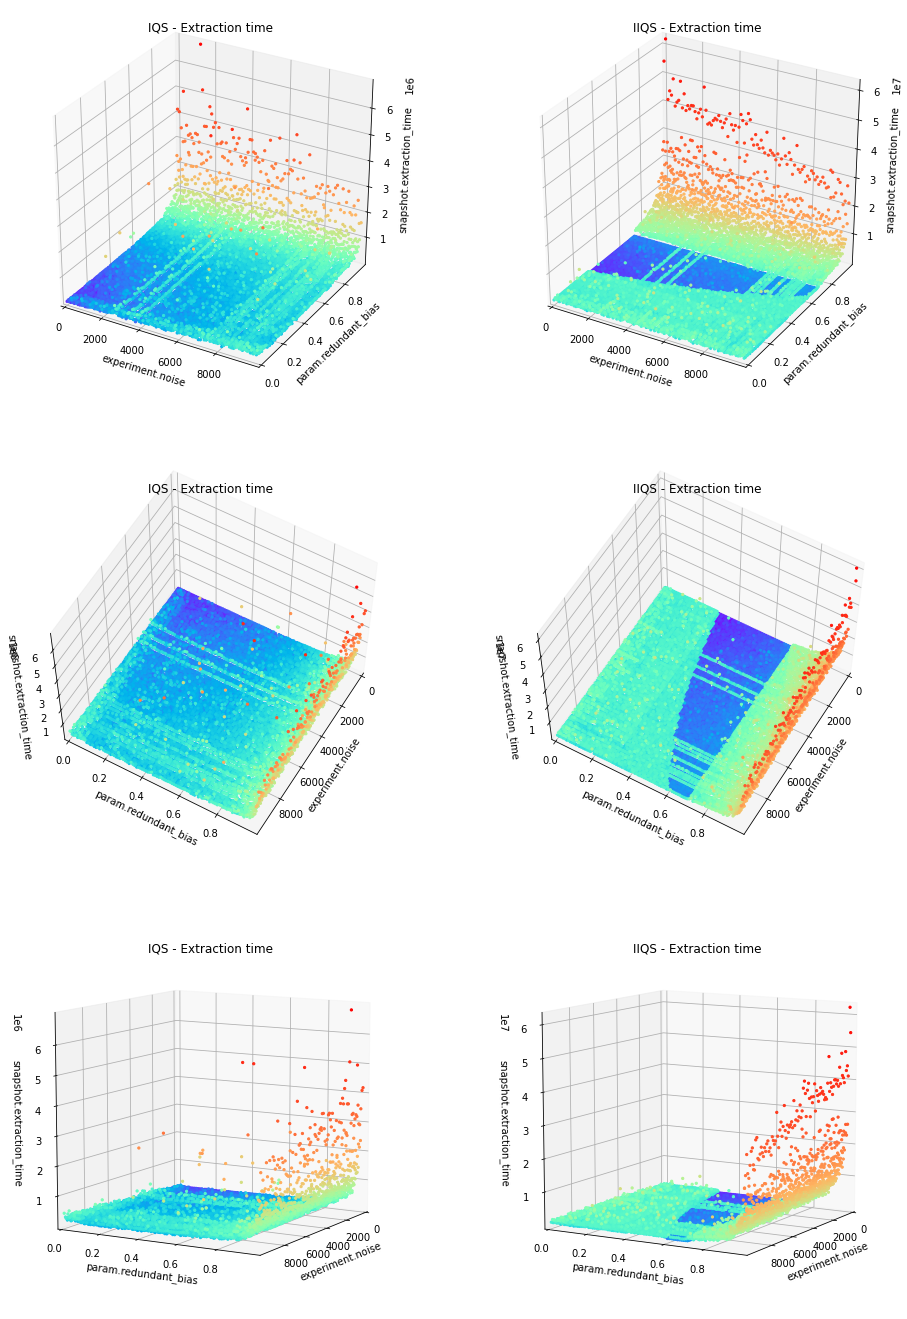
\includegraphics[width=0.8\textwidth]{./fragments/04_experimental_execution/images/01_basebenchmark_06_noise_bias.png}
    %\caption{Benchmark for random case. IQS and IIQS executions are shown on the first and second columns respectively.}
    \caption{Benchmark for randomly sorted sequence with repeated elements $1\times10^4$ elements. IQS and IIQS executions are shown on the first and second column respectively. All extractions are being shown using a linear scale.}
    \label{FIG:BENCHMARK_06_NOISE_BIAS}
\end{figure}

For our first observation we limit the result to only examine the first extraction performed by IQS, as it is already known that it is the most compute intensive operation in this algorithm. Then, we can observe in Figure \ref{FIG:BENCHMARK_06_NOISE_BIAS} that both the noise amount and the bias over the partition have a huge impact when extracting the first element in the sequence which is also different for both implementations of the algorithm.

% By examining the extra information provided by our first experiment, there are two noticeable details on the effect of biasing the selection of the resulting pivot. 
There are some interesting effects of the sequence noise for the repeating case instance. IQS shows the best performance as the noise decreases but also as the pivot bias is more inclined towards selecting the smaller elements. But this effect it is only an illusion generated by the same case depicted on Figure~\ref{FIG:BENCHMARK_02_ASC_CASE}, as less noise is found in the sequence, the greater the chance to select as pivot an element belonging to the repeating portion of the sequence, hence the bias effect studied on IQS for the partition comes into full effect. Both changing the bias towards greater values and to increase the noise contributes to increase the extraction time, it is clear that the bias has a greater effect than noise. 

Then something interesting happens on IIQS, as the behaviour is not as smooth as on IQS case. There is a valley that it appears to be in function of the bias, which for certain amounts of noise in the sequence it favours their execution. This is because of a forced execution of the introspective steps. Both noise and pivot bias have a huge impact on the times that this step is executed, hence, aditional $O(n)$ time is consumed on the iteration when the noise exceeds IIQS fixed $\alpha$ and $\beta$ constraints~\cite{7416566}. In the same fashion as our previous observations, the fact that this effect decreases when inducing more noise is related to the probability of randomly selecting a pivot which belong to a repeated portion of the array. When this happens we notice a great reduction of the running time, which suggest that we should adjust our pivot bias to match our $\alpha$ and $\beta$ values in order to get the best performance.

\begin{figure}[!ht]
    \centering
    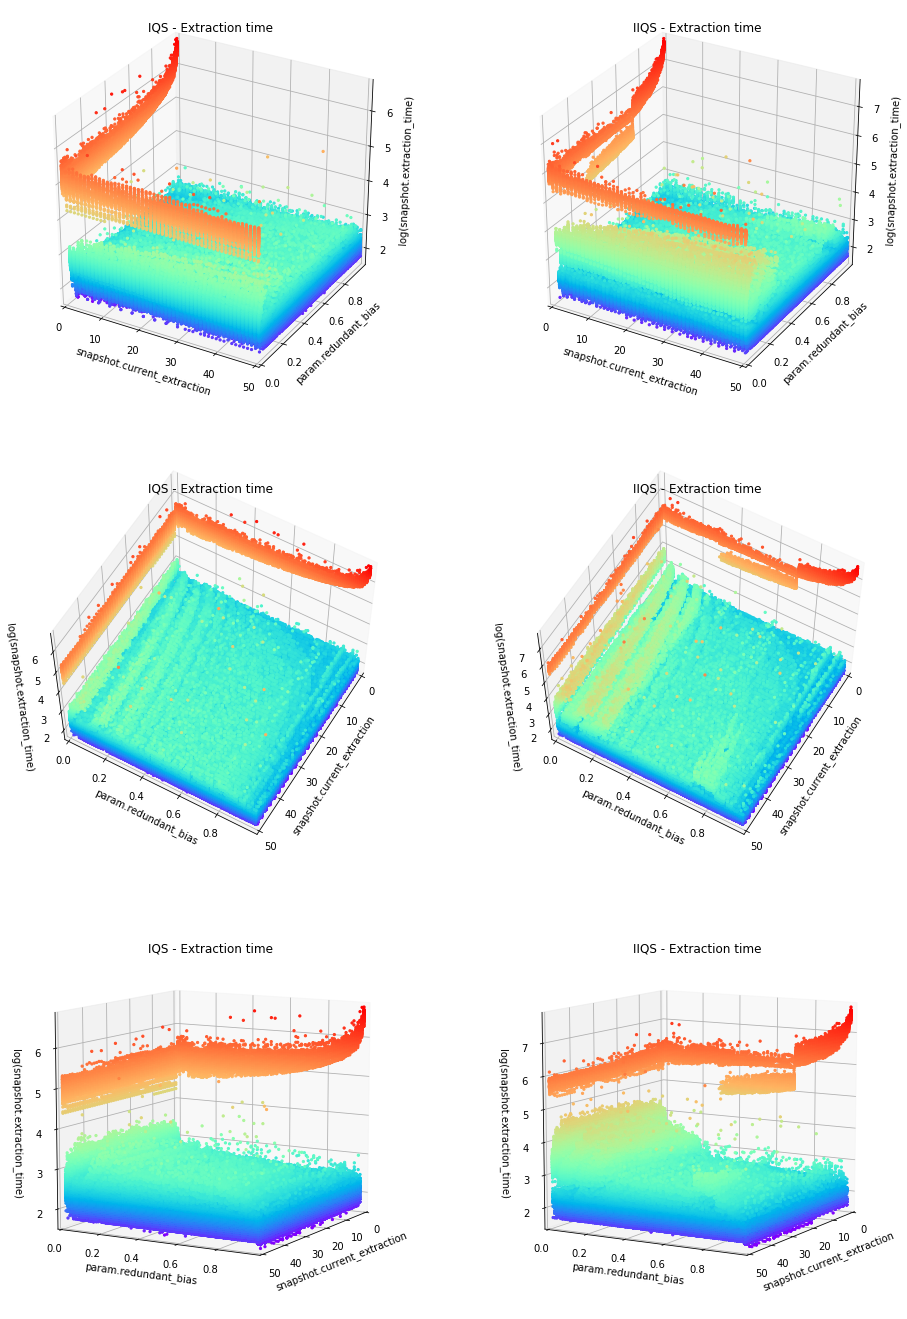
\includegraphics[width=0.8\textwidth]{./fragments/04_experimental_execution/images/01_basebenchmark_07_extraction_bias.png}
    %\caption{Benchmark for random case. IQS and IIQS executions are shown on the first and second columns respectively.}
    \caption{Benchmark for randomly sorted sequence with repeated elements $1\times10^4$ elements. IQS and IIQS executions are shown on the first and second column respectively. All extractions using a symlog scale.}
    \label{FIG:BENCHMARK_07_NOISE_BIAS}
\end{figure}

Let us assume now that there is no noise in our sequence, in order to match a best case execution for IQS. Then by looking the effects of the pivot bias against the subsequent extractions in Figure~\ref{FIG:BENCHMARK_07_NOISE_BIAS} we notice setting our pivot bias towards the leftmost elements in the pivot segment is not a good idea. When there is only one class and there is no noise in the sequence, the extractions become more costly as the pivot bias deviates from the ideal $0.5$ value. This holds for both the first extraction and the subsequent ones. Also, it does clearly state that fixing the pivot bias to one extreme or another is not a good idea. 

For IIQS the same rules apply, with the difference that there is a boost of performance when the bias belongs to the $[\alpha,\beta]$ range, as the introspective step rearranges the element and this ends being more cheaper in some cases than to continue the partition stage blindfolded.

\FloatBarrier
\section{Median selection}
\subsection{Current median selection approach}
\subsection{Iterative median of medians}
\subsection{Effects on future calls}
\subsection{Suggestions}


\section{Stack structure}
\subsection{Stack performance}
\subsection{Paired stack performance}
\subsection{Performance comparison for repeated sequences and unique sequences}
\subsection{Stack management comparison for repeated sequences and unique sequences}

\chapter{Pilot experiments}

\section{Experimental Setup}


\section{Base benchmarking}
In experimental algorithms, the first step before engaging into a optimization job is to benchmark our current solutions in order to formulate our hypothesis and expectations. In this case we will check the behaivour of base implementations IQS and IIQS to understand better what IQS and IIQS is, what is happening when a worst case arises and to devise the next steps of this experimental development.

\subsection{Average and worst case}
RESULTS, A TON OF CHARTS AND DISCUSSION
\subsection{Influence of presortedness}
RESULTS, A TON OF CHARTS AND DISCUSSION
\subsection{Influence of repeated elements}
RESULTS, A TON OF CHARTS AND DISCUSSION



% REMEMBER TO ANSWER THEESE QUESTIONS:

% Is IIQS execution for repeated elements an instance of IQS worstcase?
% Does presortedness affect (I)IQS running time?
% Does the size of the elements stored in the stack affect its performance?
% It is worth to use iterative versions of BFPRT as approximate median selection?
% Are the average cases for repeated and non repeated classes the same?} %rewrit
% Can we tune (I)IQS to support repeated cases without affecting its average running time?
\section{Partitioning Schemes}

\subsection{Rationale}
Before diving into the results for this experiment, we will now explain two partition strategies to take into consideration before designing our first experiment and our second algorithm modification in order to understand the modifications made to IQS.

\subsection{Partition schemes}
As explained before in~\ref{SEC:INCREMENTAL_SORTING}, partition algorithms play a fundamental role on sorting algorithms like QuickSort. But partition algorithms can use different schemes in order to partition the array into two sections, depending on which properties of the process we want to optimise.

\subsection{Lomuto's partition scheme}

The most identificable feature of this algorithm is that it uses the last element as the pivot for partitioning the array, which makes suitable for shuffled sequences but when the sequence follows some of the first disorder metrics seen in~\ref{SEC:MEASURING_DISORDER} it tends to bias the performance of this partition scheme.

This algorithm is commonly referenced as the easiest way to partition an array, given it is low complexity.
o
\begin{algorithm}
\caption{Lomuto Partition}\label{ALG:LOMUTO_PARTITION}
\begin{algorithmic}[1]
    \Procedure{$lomuto$}{$A, p, r$}
    \State $x \gets A_r$
    \State $i \gets p-1$
    \For{$j \in [p, r - 1]$}
    \If{$A_j \leq x$}
        \State $i \gets i + i$
        \State $swap(A_i, A_j)$
    \EndIf
    \EndFor
    \State $swap(A_{i+1}, A_r)$
    \State \Return $i + 1$
    \EndProcedure
\end{algorithmic}
\end{algorithm}

\subsection{Hoare's partition scheme}
Hoare's partition scheme takes another approach at partitioning elements by using two indices which converge into the postition of the pivot chosen at the beggining. When it comes to sort a set of elements it works faster than Lomuto's implementation and it's more stable. and given that the pivot can be chosen randomly, the introduction of randomness helps to ease biased pivot selections.

\begin{algorithm}
\caption{Hoare's Partition}\label{ALG:HOARE_PARTITION}
\begin{algorithmic}[1]
    \Procedure{$hoare$}{$A, p, r$}
    \State $x \gets A_p$
    \State $i \gets p-1$
    \State $j \gets r+1$
    \While{$true$}
        \Do 
            \State $j \gets j - 1$
        \doWhile{$A_j \leq x$}

        \Do 
            \State $i \gets i + 1$
        \doWhile{$A_j \geq x$}

        \If{$i < j$}
            \State $swap(A_i, A_j)$
        \Else
            \State \Return $j$
        \EndIf
    \EndWhile
    \EndProcedure
\end{algorithmic}
\end{algorithm}

\subsection{Dutch flag problem}
Both of the aforementioned algorithms performs over sets, but when it comes to sequences, to use such partition methods fails dramatically as it treats repeated elements as unique elements. In worst case, the pivot is positioned into its corresponding place but it does not guarantee that there are no repetitions of the same element on any portion of the original sequence.

\subsection{Problem definition and solution}
Let's take as example the partitioning problem of the following two sequences:

$$ S_1={1,2,3,4,5,6,7,8,9} $$
and
$$S_2={1,2,5,5,5,5,5,8,9}$$

It's clear that if we chose $p$ equal to $5$, the element in the fifth position of $S_1$ will be the pivot on its correct place. But it's not the case for $S_2$ as we can get a pivot from the third up to the seventh position on the sequence. In this case, as all the positions are valid pivots, there is no safety guarantee that the resulting pivot will partition the array in half in order to ensure a $log_2$ decay on the problem space. Situation worsens if all the elements are repeated, as it defeats the purpose of partitioning the sequence~\cite{7416566}.

This problem is also known as the Dutch Flag problem~\cite{10.5555/550359}, which for given a sequence it partition inplace the elements lower than the pivot value, the elements equal to the pivot value and the elements greater than the pivot value and it will return the indices of the beggining and the end of the middle portion.

\begin{algorithm}
\caption{Hoare's Partition}\label{ALG:HOARE_PARTITION}
\begin{algorithmic}[1]
    \Procedure{$hoare$}{$A, p, r$}
    \State $x \gets A_p$
    \State $i \gets p-1$
    \State $j \gets r+1$
    \While{$true$}
        \Do 
            \State $j \gets j - 1$
        \doWhile{$A_j \leq x$}

        \Do 
            \State $i \gets i + 1$
        \doWhile{$A_j \geq x$}

        \If{$i < j$}
            \State $swap(A_i, A_j)$
        \Else
            \State \Return $j$
        \EndIf
    \EndWhile
    \EndProcedure
\end{algorithmic}
\end{algorithm}

\subsection{Integration into IQS as base implementation}

SECTION WITH RESULTS HERE!!!

As it can be seen, there no noticeable difference between experimental complexities of implementations for three-way partitioning and standard partitioning algorithms. As such, from now on we will use \textit{three-waw-partition} as our default implementation for the partitioning stage. This will allow us to contrast results between IQS and IIQS with such modifications using both repeated and non repeated elements as dataset inputs.







\section{Influence of pivot selection}

In this experiment we establish a baseline for selecting pivots on partition-based sorting algorithms. While it is commonly known that randomized approaches are the most effective way of dealing with unknown distributions~\cite{estivil92}, in this approach we want to confirm if by biasing the selection on the partitioning stages of the algorithms have any direct influence over its running time.

\subsection{Understanding pivot bias}

As explained before in Section~\ref{SECTION:PARTITIONING_SCHEMES}, all partition based algorithms are based in the idea of generating two equal sized partitions, which contributes to a continuous decrease by a factor of 2 on each iteration. Under normal circumstances, it is expected that $log_2(n)$ partition operations are executed for a given sequence of $n$ size.

But this assumption only yields when there is only one pivot to select. Meaning that there is a single element which divides both partitions generated by the algorithm, so for the case of a \emph{three-way-partition} it does not apply. Let us take a example of a sequence $S$ of size $n$ which contains $n$ unique integer elements. So, by induction on the integer number definition, each element if used as pivot for a partition can only yield one and only one pair of partition sets on $S$.

When repeated elements are found on $S$ we face a problem with the definition itself of partition presented in Section~\ref{SUBSECITON:PARTITIONING_PROBLEM}, as there is no guarantee that the partitioned element is present or not in the resulting array. Using a three-way partitioning element does not solve the problem of reducing the search space and in this regard we have the following two options:

\begin{itemize}
    \item Group the repeated elements and threat that set of repeated element as they were a unique element on $S$ --- we discuss this approach on Section~\ref{SECTION:STACK_STRUCTURE}.
    \item Preserve the elements into the array and we apply a set of rules to choose which element deliver as our pivot.
\end{itemize}

This makes a lot of sense when revisiting the plot at Figure~\ref{FIG:BENCHMARK_05_CLASSES}, as the more predominant is a certain class in a sequence, the less important becomes the pivot value selected but their final position.

\subsection{Effects on the partitioning}

Let us consider the pivot bias as a rational number $p_b \in [0,1]$. This bias allows us to map to indexes in $S$ to a floating point representation by assuming $S_i = \lfloor n\cdot p_{b}  \rfloor, \forall ~i~ \in[0,\norm{S}($. In colloqual terms, this means that a index of $0.0$ means that the returned pivot belongs to the leftmost index of the middle segment, a value of $0.5$ a pivot in the middle of the segment and $1.0$ the rightmost element, asumming that the elements are sorted in a ascending fashion.

\begin{figure}[!ht]
    \centering
    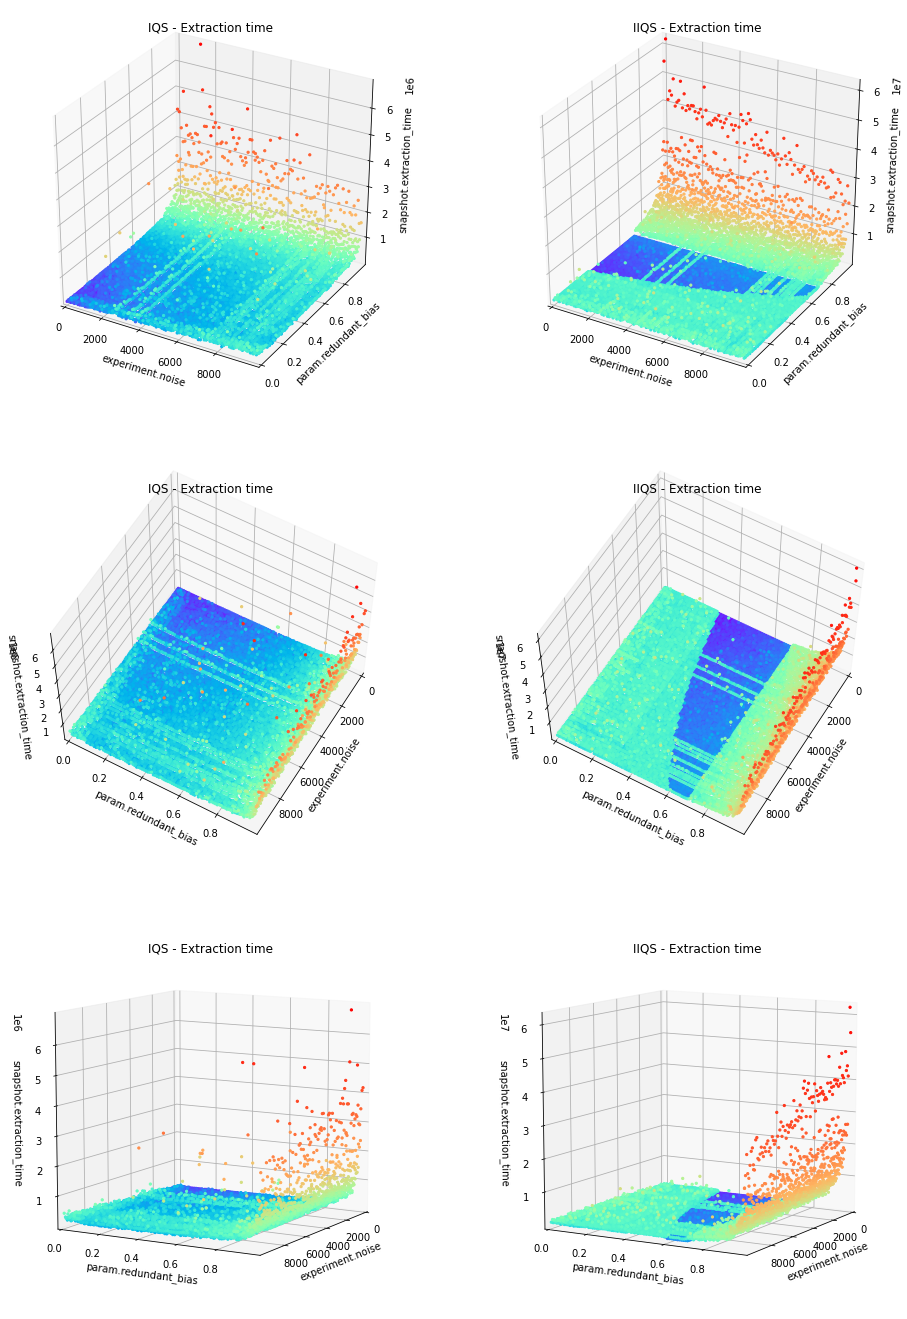
\includegraphics[width=0.8\textwidth]{./fragments/04_experimental_execution/images/01_basebenchmark_06_noise_bias.png}
    %\caption{Benchmark for random case. IQS and IIQS executions are shown on the first and second columns respectively.}
    \caption{Benchmark for randomly sorted sequence with repeated elements $1\times10^4$ elements. IQS and IIQS executions are shown on the first and second column respectively. All extractions are being shown using a linear scale.}
    \label{FIG:BENCHMARK_06_NOISE_BIAS}
\end{figure}

For our first observation we limit the result to only examine the first extraction performed by IQS, as it is already known that it is the most compute intensive operation in this algorithm. Then, we can observe in Figure \ref{FIG:BENCHMARK_06_NOISE_BIAS} that both the noise amount and the bias over the partition have a huge impact when extracting the first element in the sequence which is also different for both implementations of the algorithm.

% By examining the extra information provided by our first experiment, there are two noticeable details on the effect of biasing the selection of the resulting pivot. 
There are some interesting effects of the sequence noise for the repeating case instance. IQS shows the best performance as the noise decreases but also as the pivot bias is more inclined towards selecting the smaller elements. But this effect it is only an illusion generated by the same case depicted on Figure~\ref{FIG:BENCHMARK_02_ASC_CASE}, as less noise is found in the sequence, the greater the chance to select as pivot an element belonging to the repeating portion of the sequence, hence the bias effect studied on IQS for the partition comes into full effect. Both changing the bias towards greater values and to increase the noise contributes to increase the extraction time, it is clear that the bias has a greater effect than noise. 

Then something interesting happens on IIQS, as the behaviour is not as smooth as on IQS case. There is a valley that it appears to be in function of the bias, which for certain amounts of noise in the sequence it favours their execution. This is because of a forced execution of the introspective steps. Both noise and pivot bias have a huge impact on the times that this step is executed, hence, aditional $O(n)$ time is consumed on the iteration when the noise exceeds IIQS fixed $\alpha$ and $\beta$ constraints~\cite{7416566}. In the same fashion as our previous observations, the fact that this effect decreases when inducing more noise is related to the probability of randomly selecting a pivot which belong to a repeated portion of the array. When this happens we notice a great reduction of the running time, which suggest that we should adjust our pivot bias to match our $\alpha$ and $\beta$ values in order to get the best performance.

\begin{figure}[!ht]
    \centering
    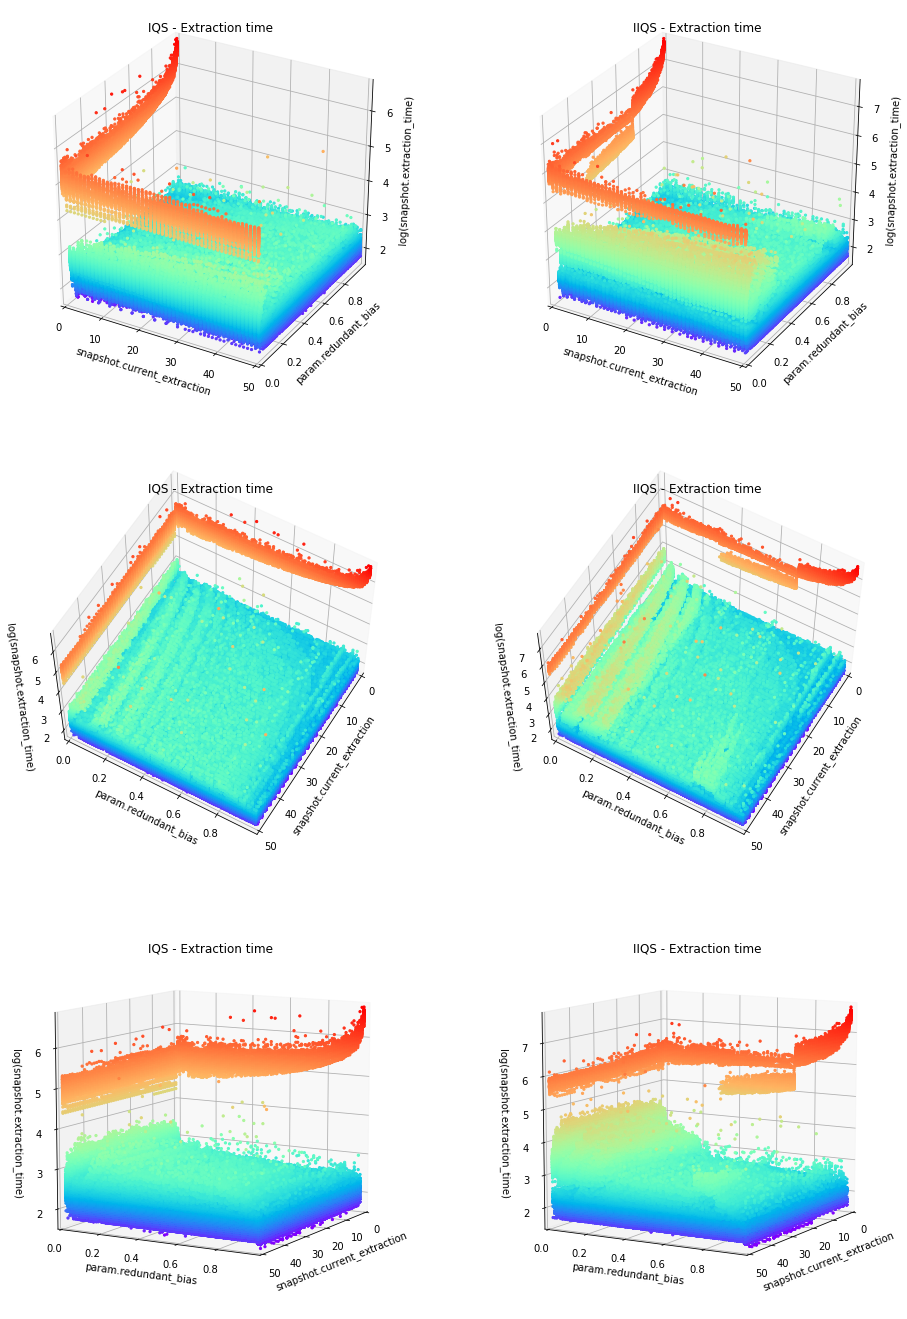
\includegraphics[width=0.8\textwidth]{./fragments/04_experimental_execution/images/01_basebenchmark_07_extraction_bias.png}
    %\caption{Benchmark for random case. IQS and IIQS executions are shown on the first and second columns respectively.}
    \caption{Benchmark for randomly sorted sequence with repeated elements $1\times10^4$ elements. IQS and IIQS executions are shown on the first and second column respectively. All extractions using a symlog scale.}
    \label{FIG:BENCHMARK_07_NOISE_BIAS}
\end{figure}

Let us assume now that there is no noise in our sequence, in order to match a best case execution for IQS. Then by looking the effects of the pivot bias against the subsequent extractions in Figure~\ref{FIG:BENCHMARK_07_NOISE_BIAS} we notice setting our pivot bias towards the leftmost elements in the pivot segment is not a good idea. When there is only one class and there is no noise in the sequence, the extractions become more costly as the pivot bias deviates from the ideal $0.5$ value. This holds for both the first extraction and the subsequent ones. Also, it does clearly state that fixing the pivot bias to one extreme or another is not a good idea. 

For IIQS the same rules apply, with the difference that there is a boost of performance when the bias belongs to the $[\alpha,\beta]$ range, as the introspective step rearranges the element and this ends being more cheaper in some cases than to continue the partition stage blindfolded.

\FloatBarrier
\section{Median selection}
\subsection{Current median selection approach}
\subsection{Iterative median of medians}
\subsection{Effects on future calls}
\subsection{Suggestions}


\section{Stack structure}
\subsection{Stack performance}
\subsection{Paired stack performance}
\subsection{Performance comparison for repeated sequences and unique sequences}
\subsection{Stack management comparison for repeated sequences and unique sequences}

\chapter{Pilot experiments}

\section{Experimental Setup}


\section{Base benchmarking}
In experimental algorithms, the first step before engaging into a optimization job is to benchmark our current solutions in order to formulate our hypothesis and expectations. In this case we will check the behaivour of base implementations IQS and IIQS to understand better what IQS and IIQS is, what is happening when a worst case arises and to devise the next steps of this experimental development.

\subsection{Average and worst case}
RESULTS, A TON OF CHARTS AND DISCUSSION
\subsection{Influence of presortedness}
RESULTS, A TON OF CHARTS AND DISCUSSION
\subsection{Influence of repeated elements}
RESULTS, A TON OF CHARTS AND DISCUSSION



% REMEMBER TO ANSWER THEESE QUESTIONS:

% Is IIQS execution for repeated elements an instance of IQS worstcase?
% Does presortedness affect (I)IQS running time?
% Does the size of the elements stored in the stack affect its performance?
% It is worth to use iterative versions of BFPRT as approximate median selection?
% Are the average cases for repeated and non repeated classes the same?} %rewrit
% Can we tune (I)IQS to support repeated cases without affecting its average running time?
\section{Partitioning Schemes}

\subsection{Rationale}
Before diving into the results for this experiment, we will now explain two partition strategies to take into consideration before designing our first experiment and our second algorithm modification in order to understand the modifications made to IQS.

\subsection{Partition schemes}
As explained before in~\ref{SEC:INCREMENTAL_SORTING}, partition algorithms play a fundamental role on sorting algorithms like QuickSort. But partition algorithms can use different schemes in order to partition the array into two sections, depending on which properties of the process we want to optimise.

\subsection{Lomuto's partition scheme}

The most identificable feature of this algorithm is that it uses the last element as the pivot for partitioning the array, which makes suitable for shuffled sequences but when the sequence follows some of the first disorder metrics seen in~\ref{SEC:MEASURING_DISORDER} it tends to bias the performance of this partition scheme.

This algorithm is commonly referenced as the easiest way to partition an array, given it is low complexity.
o
\begin{algorithm}
\caption{Lomuto Partition}\label{ALG:LOMUTO_PARTITION}
\begin{algorithmic}[1]
    \Procedure{$lomuto$}{$A, p, r$}
    \State $x \gets A_r$
    \State $i \gets p-1$
    \For{$j \in [p, r - 1]$}
    \If{$A_j \leq x$}
        \State $i \gets i + i$
        \State $swap(A_i, A_j)$
    \EndIf
    \EndFor
    \State $swap(A_{i+1}, A_r)$
    \State \Return $i + 1$
    \EndProcedure
\end{algorithmic}
\end{algorithm}

\subsection{Hoare's partition scheme}
Hoare's partition scheme takes another approach at partitioning elements by using two indices which converge into the postition of the pivot chosen at the beggining. When it comes to sort a set of elements it works faster than Lomuto's implementation and it's more stable. and given that the pivot can be chosen randomly, the introduction of randomness helps to ease biased pivot selections.

\begin{algorithm}
\caption{Hoare's Partition}\label{ALG:HOARE_PARTITION}
\begin{algorithmic}[1]
    \Procedure{$hoare$}{$A, p, r$}
    \State $x \gets A_p$
    \State $i \gets p-1$
    \State $j \gets r+1$
    \While{$true$}
        \Do 
            \State $j \gets j - 1$
        \doWhile{$A_j \leq x$}

        \Do 
            \State $i \gets i + 1$
        \doWhile{$A_j \geq x$}

        \If{$i < j$}
            \State $swap(A_i, A_j)$
        \Else
            \State \Return $j$
        \EndIf
    \EndWhile
    \EndProcedure
\end{algorithmic}
\end{algorithm}

\subsection{Dutch flag problem}
Both of the aforementioned algorithms performs over sets, but when it comes to sequences, to use such partition methods fails dramatically as it treats repeated elements as unique elements. In worst case, the pivot is positioned into its corresponding place but it does not guarantee that there are no repetitions of the same element on any portion of the original sequence.

\subsection{Problem definition and solution}
Let's take as example the partitioning problem of the following two sequences:

$$ S_1={1,2,3,4,5,6,7,8,9} $$
and
$$S_2={1,2,5,5,5,5,5,8,9}$$

It's clear that if we chose $p$ equal to $5$, the element in the fifth position of $S_1$ will be the pivot on its correct place. But it's not the case for $S_2$ as we can get a pivot from the third up to the seventh position on the sequence. In this case, as all the positions are valid pivots, there is no safety guarantee that the resulting pivot will partition the array in half in order to ensure a $log_2$ decay on the problem space. Situation worsens if all the elements are repeated, as it defeats the purpose of partitioning the sequence~\cite{7416566}.

This problem is also known as the Dutch Flag problem~\cite{10.5555/550359}, which for given a sequence it partition inplace the elements lower than the pivot value, the elements equal to the pivot value and the elements greater than the pivot value and it will return the indices of the beggining and the end of the middle portion.

\begin{algorithm}
\caption{Hoare's Partition}\label{ALG:HOARE_PARTITION}
\begin{algorithmic}[1]
    \Procedure{$hoare$}{$A, p, r$}
    \State $x \gets A_p$
    \State $i \gets p-1$
    \State $j \gets r+1$
    \While{$true$}
        \Do 
            \State $j \gets j - 1$
        \doWhile{$A_j \leq x$}

        \Do 
            \State $i \gets i + 1$
        \doWhile{$A_j \geq x$}

        \If{$i < j$}
            \State $swap(A_i, A_j)$
        \Else
            \State \Return $j$
        \EndIf
    \EndWhile
    \EndProcedure
\end{algorithmic}
\end{algorithm}

\subsection{Integration into IQS as base implementation}

SECTION WITH RESULTS HERE!!!

As it can be seen, there no noticeable difference between experimental complexities of implementations for three-way partitioning and standard partitioning algorithms. As such, from now on we will use \textit{three-waw-partition} as our default implementation for the partitioning stage. This will allow us to contrast results between IQS and IIQS with such modifications using both repeated and non repeated elements as dataset inputs.







\section{Influence of pivot selection}

In this experiment we establish a baseline for selecting pivots on partition-based sorting algorithms. While it is commonly known that randomized approaches are the most effective way of dealing with unknown distributions~\cite{estivil92}, in this approach we want to confirm if by biasing the selection on the partitioning stages of the algorithms have any direct influence over its running time.

\subsection{Understanding pivot bias}

As explained before in Section~\ref{SECTION:PARTITIONING_SCHEMES}, all partition based algorithms are based in the idea of generating two equal sized partitions, which contributes to a continuous decrease by a factor of 2 on each iteration. Under normal circumstances, it is expected that $log_2(n)$ partition operations are executed for a given sequence of $n$ size.

But this assumption only yields when there is only one pivot to select. Meaning that there is a single element which divides both partitions generated by the algorithm, so for the case of a \emph{three-way-partition} it does not apply. Let us take a example of a sequence $S$ of size $n$ which contains $n$ unique integer elements. So, by induction on the integer number definition, each element if used as pivot for a partition can only yield one and only one pair of partition sets on $S$.

When repeated elements are found on $S$ we face a problem with the definition itself of partition presented in Section~\ref{SUBSECITON:PARTITIONING_PROBLEM}, as there is no guarantee that the partitioned element is present or not in the resulting array. Using a three-way partitioning element does not solve the problem of reducing the search space and in this regard we have the following two options:

\begin{itemize}
    \item Group the repeated elements and threat that set of repeated element as they were a unique element on $S$ --- we discuss this approach on Section~\ref{SECTION:STACK_STRUCTURE}.
    \item Preserve the elements into the array and we apply a set of rules to choose which element deliver as our pivot.
\end{itemize}

This makes a lot of sense when revisiting the plot at Figure~\ref{FIG:BENCHMARK_05_CLASSES}, as the more predominant is a certain class in a sequence, the less important becomes the pivot value selected but their final position.

\subsection{Effects on the partitioning}

Let us consider the pivot bias as a rational number $p_b \in [0,1]$. This bias allows us to map to indexes in $S$ to a floating point representation by assuming $S_i = \lfloor n\cdot p_{b}  \rfloor, \forall ~i~ \in[0,\norm{S}($. In colloqual terms, this means that a index of $0.0$ means that the returned pivot belongs to the leftmost index of the middle segment, a value of $0.5$ a pivot in the middle of the segment and $1.0$ the rightmost element, asumming that the elements are sorted in a ascending fashion.

\begin{figure}[!ht]
    \centering
    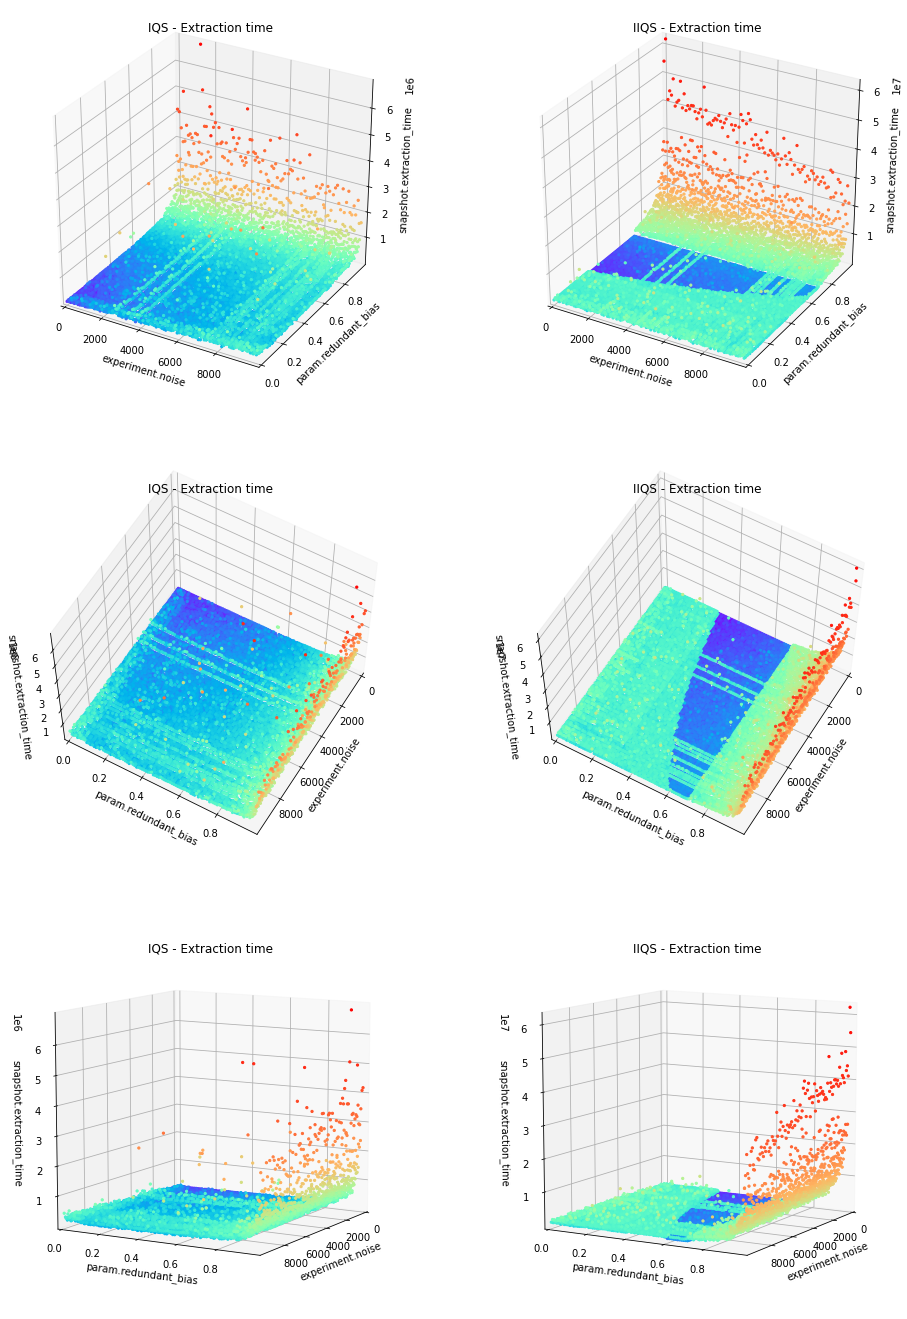
\includegraphics[width=0.8\textwidth]{./fragments/04_experimental_execution/images/01_basebenchmark_06_noise_bias.png}
    %\caption{Benchmark for random case. IQS and IIQS executions are shown on the first and second columns respectively.}
    \caption{Benchmark for randomly sorted sequence with repeated elements $1\times10^4$ elements. IQS and IIQS executions are shown on the first and second column respectively. All extractions are being shown using a linear scale.}
    \label{FIG:BENCHMARK_06_NOISE_BIAS}
\end{figure}

For our first observation we limit the result to only examine the first extraction performed by IQS, as it is already known that it is the most compute intensive operation in this algorithm. Then, we can observe in Figure \ref{FIG:BENCHMARK_06_NOISE_BIAS} that both the noise amount and the bias over the partition have a huge impact when extracting the first element in the sequence which is also different for both implementations of the algorithm.

% By examining the extra information provided by our first experiment, there are two noticeable details on the effect of biasing the selection of the resulting pivot. 
There are some interesting effects of the sequence noise for the repeating case instance. IQS shows the best performance as the noise decreases but also as the pivot bias is more inclined towards selecting the smaller elements. But this effect it is only an illusion generated by the same case depicted on Figure~\ref{FIG:BENCHMARK_02_ASC_CASE}, as less noise is found in the sequence, the greater the chance to select as pivot an element belonging to the repeating portion of the sequence, hence the bias effect studied on IQS for the partition comes into full effect. Both changing the bias towards greater values and to increase the noise contributes to increase the extraction time, it is clear that the bias has a greater effect than noise. 

Then something interesting happens on IIQS, as the behaviour is not as smooth as on IQS case. There is a valley that it appears to be in function of the bias, which for certain amounts of noise in the sequence it favours their execution. This is because of a forced execution of the introspective steps. Both noise and pivot bias have a huge impact on the times that this step is executed, hence, aditional $O(n)$ time is consumed on the iteration when the noise exceeds IIQS fixed $\alpha$ and $\beta$ constraints~\cite{7416566}. In the same fashion as our previous observations, the fact that this effect decreases when inducing more noise is related to the probability of randomly selecting a pivot which belong to a repeated portion of the array. When this happens we notice a great reduction of the running time, which suggest that we should adjust our pivot bias to match our $\alpha$ and $\beta$ values in order to get the best performance.

\begin{figure}[!ht]
    \centering
    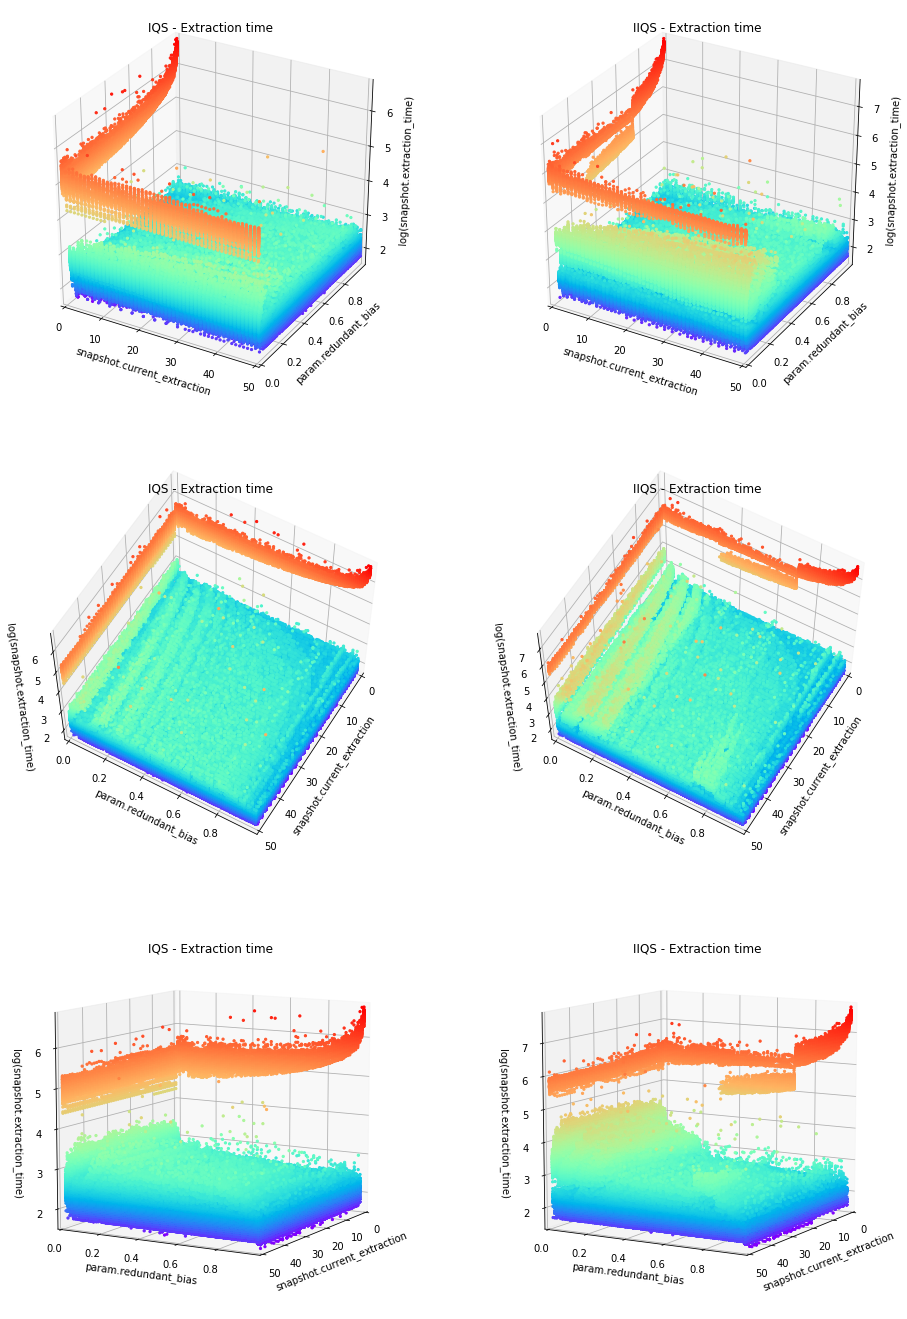
\includegraphics[width=0.8\textwidth]{./fragments/04_experimental_execution/images/01_basebenchmark_07_extraction_bias.png}
    %\caption{Benchmark for random case. IQS and IIQS executions are shown on the first and second columns respectively.}
    \caption{Benchmark for randomly sorted sequence with repeated elements $1\times10^4$ elements. IQS and IIQS executions are shown on the first and second column respectively. All extractions using a symlog scale.}
    \label{FIG:BENCHMARK_07_NOISE_BIAS}
\end{figure}

Let us assume now that there is no noise in our sequence, in order to match a best case execution for IQS. Then by looking the effects of the pivot bias against the subsequent extractions in Figure~\ref{FIG:BENCHMARK_07_NOISE_BIAS} we notice setting our pivot bias towards the leftmost elements in the pivot segment is not a good idea. When there is only one class and there is no noise in the sequence, the extractions become more costly as the pivot bias deviates from the ideal $0.5$ value. This holds for both the first extraction and the subsequent ones. Also, it does clearly state that fixing the pivot bias to one extreme or another is not a good idea. 

For IIQS the same rules apply, with the difference that there is a boost of performance when the bias belongs to the $[\alpha,\beta]$ range, as the introspective step rearranges the element and this ends being more cheaper in some cases than to continue the partition stage blindfolded.

\FloatBarrier
\section{Median selection}
\subsection{Current median selection approach}
\subsection{Iterative median of medians}
\subsection{Effects on future calls}
\subsection{Suggestions}


\section{Stack structure}
\subsection{Stack performance}
\subsection{Paired stack performance}
\subsection{Performance comparison for repeated sequences and unique sequences}
\subsection{Stack management comparison for repeated sequences and unique sequences}


\chapter{Summary}
% \chapter{Experiments}
% \section{Experimental setup}
% \section{Experimental results}
% \section{Metrics and indicators}
% \subsection{Local entropy decay}
% \subsection{BFPRT executions}
% \subsection{Partitioner executions}

% \section{Tunning}
% \subsection{Data generation and execution control}


% %% contenido del segundo capítulo
% \chapter{Segundo Capítulo}
% Sólo para probar algunas cosas como las referencias.
% La primera cita es a Lamport~\cite{lamport79}.
% La segunda cita es para Lamport nuevamente~\cite{lamport78}.
% La última cita es para Keleher \emph{et al.}~\cite{keleher92}.


% %% contenido del tercer capítulo
% \chapter{Tercer Capítulo}
% Sólo para incluir figuras y tablas.
% \begin{figure}[h]
%   \vspace*{1cm}
%   \includegraphics[bb=0 0 640 480, width=.5\linewidth]{latexlogo.png}
%   \vspace*{1cm}
%   \caption{La primera figura de la memoria}
% \end{figure}
% \begin{table}[h]
%   \vspace*{1cm}
%   (aqui debiera ir la tabla)
%   \vspace*{1cm}
%   \caption{La primera tabla de la memoria}
% \end{table}


%% ambiente glosario
\begin{glosario}
  \item[El primer término:] Este es el significado del primer término, realmente no se bien lo que significa pero podría haberlo averiguado si hubiese tenido un poco mas de tiempo.
  \item[El segundo término:] Este si se lo que significa pero me da lata escribirlo...
\end{glosario}


%% genera las referencias
\bibliography{refs}


%% comienzo de la parte de anexos
\appendixpart

%% contenido del primer anexo
\appendix{El Primer Anexo}
Aquí va el texto del primer anexo...

\section{La primera sección del primer anexo}
Aquí va el texto de la primera sección del primer anexo...

\section{La segunda sección del primer anexo}
Aquí va el texto de la segunda sección del primer anexo...

\subsection{La primera subsección de la segunda sección del primer anexo}


%% contenido del segundo anexo
\appendix{El segundo Anexo}
Aquí va el texto del segundo anexo...

\section{La primera sección del segundo anexo}
Aquí va el texto de la primera sección del segundo anexo...

%% fin
\end{document}



